%%%%%%%%%%%%%%%%%%%%%%%%%%%%%%%%%%%%%%%%%%%%%%%%%%%%%%%%%%%%%%%%%%%%%%%%%%%%%%%%%%%%
% Template for STAT 547C final project
% Author: Ben Bloem-Reddy <benbr@stat.ubc.ca>
% Date: Oct. 18, 2019
%%%%%%%%%%%%%%%%%%%%%%%%%%%%%%%%%%%%%%%%%%%%%%%%%%%%%%%%%%%%%%%%%%%%%%%%%%%%%%%%%%%%

% Note: You will get an empty bibliography warning when compiling until you include a citation.

\documentclass[10pt, titlepage]{article}
% header.tex
% this is where you load pacakges, specify custom formats, etc.

\usepackage[left=1in,right=1in,top=0.75in,footskip=25pt]{geometry} 
% \usepackage{changepage}
\usepackage{amsmath,amsthm,amssymb,amsfonts}
\usepackage{mathtools}
% enumitem for custom lists
\usepackage{enumitem}
% Load dsfont this to get proper indicator function (bold 1) with \mathds{1}:
\usepackage{dsfont}
\usepackage{centernot}

\usepackage[usenames,dvipsnames]{xcolor}

% set up commenting code (I will use this during marking)
\definecolor{CommentColor}{rgb}{0,.50,.50}
\newcounter{margincounter}
\newcommand{\displaycounter}{{\arabic{margincounter}}}
\newcommand{\incdisplaycounter}{{\stepcounter{margincounter}\arabic{margincounter}}}
\newcommand{\COMMENT}[1]{\textcolor{CommentColor}{$\,^{(\incdisplaycounter)}$}\marginpar{\scriptsize\textcolor{CommentColor}{ {\tiny $(\displaycounter)$} #1}}}

\usepackage{appendix}

% set up graphics
\usepackage{graphicx}
\DeclareGraphicsExtensions{.pdf,.png,.jpg}
\graphicspath{ {fig/} }

\usepackage[sorting=nyt,backend=biber,bibstyle=alphabetic,citestyle=alphabetic,giveninits=true]{biblatex}

\usepackage{fancyhdr}
\pagestyle{fancy}
\setlength{\headheight}{40pt}

%%%%%%%%%%%%%%%%%%%%%%%%%%%%%%%%%%%%%%%%%%%%%%%%%%%%%%%%%%%%%%%%%%%%%%%%%%%%%%%%%%%%
% most other packages you might use should be loaded before hyperref
%%%%%%%%%%%%%%%%%%%%%%%%%%%%%%%%%%%%%%%%%%%%%%%%%%%%%%%%%%%%%%%%%%%%%%%%%%%%%%%%%%%%

% Set up hyperlinks:
\definecolor{RefColor}{rgb}{0,0,.65}
\usepackage[colorlinks,linkcolor=RefColor,citecolor=RefColor,urlcolor=RefColor]{hyperref}

\usepackage[capitalize]{cleveref}
\crefname{appsec}{Appendix}{Appendices} % you can tell cleveref what to call things
% defs.tex
% this is where you define custom notation, commands, etc.


%%
% full alphabets of different styles
%%

% bf series
\def\bfA{\mathbf{A}}
\def\bfB{\mathbf{B}}
\def\bfC{\mathbf{C}}
\def\bfD{\mathbf{D}}
\def\bfE{\mathbf{E}}
\def\bfF{\mathbf{F}}
\def\bfG{\mathbf{G}}
\def\bfH{\mathbf{H}}
\def\bfI{\mathbf{I}}
\def\bfJ{\mathbf{J}}
\def\bfK{\mathbf{K}}
\def\bfL{\mathbf{L}}
\def\bfM{\mathbf{M}}
\def\bfN{\mathbf{N}}
\def\bfO{\mathbf{O}}
\def\bfP{\mathbf{P}}
\def\bfQ{\mathbf{Q}}
\def\bfR{\mathbf{R}}
\def\bfS{\mathbf{S}}
\def\bfT{\mathbf{T}}
\def\bfU{\mathbf{U}}
\def\bfV{\mathbf{V}}
\def\bfW{\mathbf{W}}
\def\bfX{\mathbf{X}}
\def\bfY{\mathbf{Y}}
\def\bfZ{\mathbf{Z}}

% bb series
\def\bbA{\mathbb{A}}
\def\bbB{\mathbb{B}}
\def\bbC{\mathbb{C}}
\def\bbD{\mathbb{D}}
\def\bbE{\mathbb{E}}
\def\bbF{\mathbb{F}}
\def\bbG{\mathbb{G}}
\def\bbH{\mathbb{H}}
\def\bbI{\mathbb{I}}
\def\bbJ{\mathbb{J}}
\def\bbK{\mathbb{K}}
\def\bbL{\mathbb{L}}
\def\bbM{\mathbb{M}}
\def\bbN{\mathbb{N}}
\def\bbO{\mathbb{O}}
\def\bbP{\mathbb{P}}
\def\bbQ{\mathbb{Q}}
\def\bbR{\mathbb{R}}
\def\bbS{\mathbb{S}}
\def\bbT{\mathbb{T}}
\def\bbU{\mathbb{U}}
\def\bbV{\mathbb{V}}
\def\bbW{\mathbb{W}}
\def\bbX{\mathbb{X}}
\def\bbY{\mathbb{Y}}
\def\bbZ{\mathbb{Z}}

% cal series
\def\calA{\mathcal{A}}
\def\calB{\mathcal{B}}
\def\calC{\mathcal{C}}
\def\calD{\mathcal{D}}
\def\calE{\mathcal{E}}
\def\calF{\mathcal{F}}
\def\calG{\mathcal{G}}
\def\calH{\mathcal{H}}
\def\calI{\mathcal{I}}
\def\calJ{\mathcal{J}}
\def\calK{\mathcal{K}}
\def\calL{\mathcal{L}}
\def\calM{\mathcal{M}}
\def\calN{\mathcal{N}}
\def\calO{\mathcal{O}}
\def\calP{\mathcal{P}}
\def\calQ{\mathcal{Q}}
\def\calR{\mathcal{R}}
\def\calS{\mathcal{S}}
\def\calT{\mathcal{T}}
\def\calU{\mathcal{U}}
\def\calV{\mathcal{V}}
\def\calW{\mathcal{W}}
\def\calX{\mathcal{X}}
\def\calY{\mathcal{Y}}
\def\calZ{\mathcal{Z}}


%%%%%%%%%%%%%%%%%%%%%%%%%%%%%%%%%%%%%%%%%%%%%%%%%%%%%%%%%%
% text short-cuts
\def\iid{i.i.d.\ } %i.i.d.
\def\ie{i.e.\ }
\def\eg{e.g.\ }
\def\Polya{P\'{o}lya\ }
%%%%%%%%%%%%%%%%%%%%%%%%%%%%%%%%%%%%%%%%%%%%%%%%%%%%%%%%%%

%%%%%%%%%%%%%%%%%%%%%%%%%%%%%%%%%%%%%%%%%%%%%%%%%%%%%%%%%%
% quasi-universal probabilistic and mathematical notation
% my preferences (modulo publication conventions, and clashes like random vectors):
%   vectors: bold, lowercase
%   matrices: bold, uppercase
%   operators: blackboard (e.g., \mathbb{E}), uppercase
%   sets, spaces: calligraphic, uppercase
%   random variables: normal font, uppercase
%   deterministic quantities: normal font, lowercase
%%%%%%%%%%%%%%%%%%%%%%%%%%%%%%%%%%%%%%%%%%%%%%%%%%%%%%%%%%

% operators
\def\P{\bbP} %fundamental probability
\def\E{\bbE} %expectation
% conditional expectation
\DeclarePairedDelimiterX\bigCond[2]{[}{]}{#1 \;\delimsize\vert\; #2}
\newcommand{\conditional}[3][]{\bbE_{#1}\bigCond*{#2}{#3}}
\def\Law{\mathcal{L}} %law; this is by convention in the literature
\def\indicator{\mathds{1}} % indicator function

% sets and groups
\def\borel{\calB} %Borel sets
\def\sigAlg{\calA} %sigma-algebra
\def\filtration{\calF} %filtration
\def\grp{\calG} %group

% binary relations
\def\condind{{\perp\!\!\!\perp}} %independence/conditional independence
\def\equdist{\stackrel{\text{\rm\tiny d}}{=}} %equal in distribution
\def\equas{\stackrel{\text{\rm\tiny a.s.}}{=}} %euqal amost surely
\def\simiid{\sim_{\mbox{\tiny iid}}} %sampled i.i.d

% common vectors and matrices
\def\onevec{\mathbf{1}}
\def\iden{\mathbf{I}} % identity matrix
\def\supp{\text{\rm supp}}

% misc
% floor and ceiling
\DeclarePairedDelimiter{\ceilpair}{\lceil}{\rceil}
\DeclarePairedDelimiter{\floor}{\lfloor}{\rfloor}
\newcommand{\argdot}{{\,\vcenter{\hbox{\tiny$\bullet$}}\,}} %generic argument dot
%%%%%%%%%%%%%%%%%%%%%%%%%%%%%%%%%%%%%%%%%%%%%%%%%%%%%%%%%%

%%%%%%%%%%%%%%%%%%%%%%%%%%%%%%%%%%%%%%%%%%%%%%%%%%%%%%%%%%
%% some distributions
% continuous
\def\UnifDist{\text{\rm Unif}}
\def\BetaDist{\text{\rm Beta}}
\def\ExpDist{\text{\rm Exp}}
\def\GammaDist{\text{\rm Gamma}}
% \def\GenGammaDist{\text{\rm GGa}} %Generalized Gamma

% discrete
\def\BernDist{\text{\rm Bernoulli}}
\def\BinomDist{\text{\rm Binomial}}
\def\PoissonPlus{\text{\rm Poisson}_{+}}
\def\PoissonDist{\text{\rm Poisson}}
\def\NBPlus{\text{\rm NB}_{+}}
\def\NBDist{\text{\rm NB}}
\def\GeomDist{\text{\rm Geom}}
% \def\CRP{\text{\rm CRP}}
% \def\EGP{\text{\rm EGP}}
% \def\MittagLeffler{\text{\rm ML}}
%%%%%%%%%%%%%%%%%%%%%%%%%%%%%%%%%%%%%%%%%%%%%%%%%%%%%%%%%%

%%%%%%%%%%%%%%%%%%%%%%%%%%%%%%%%%%%%%%%%%%%%%%%%%%%%%%%%%%
% Project-specific notation should go here
% (Because it's at the end of the file, it can overwrite anything that came before.)

%e.g.,
\def\Laplacian{\calL}
\def\P{\calP}

% combinatorial objects
\def\perm{\sigma} %fixed permutation
\def\Perm{\Sigma} %random permutation
\def\part{\pi} %fixed partition
\def\Part{\Pi} %random partition


%%%%%%%%%%%%%%%%%%%%%%%%%%%%%%%%%%%%%%%%%%%%%%%%%%%%%%%%%%
\newtheorem{theorem}{Theorem}[section]
\newtheorem{corollary}{Corollary}[theorem]
\newtheorem{lemma}[theorem]{Lemma}
\newtheorem{proposition}[theorem]{Proposition}
\newtheorem{definition}[theorem]{Definition}
%%%%%%%%%%%%%%%%%%%%%%%%%%%%%%%%%%%%%%%%%%%%%%%%%%%%%%%%%%%%%%%%%%%%%%%%%%%%%%%%%

% your title/author/date information go here
\title{STAT547 Final Project: A Variational Bernstein von--Mises type result} % replace with your title
\author{Johnny Xi} % replace with your name
\date{\today} % replace with your submission date
\bibliography{../../ref/STAT_547C.bib} % add the title of your bibliography file

% start of document
\begin{document}

\maketitle
% I changed all \includes to \input so that it wouldn't print on a new page 
% background section
% !TEX root = ../main.tex

% introduction

\section{Introduction}

\paragraph{} Bayesian inference is a elegant framework for statistical analysis when the analyst wishes to embed probabilistic prior beliefs into a model. These prior beliefs are then updated according to the data to produce a posterior distribution of the parameters. For much of its history, Bayesian analysis was merely a clever idea that was hindered by the analytic tractability of complex high dimensional integrals in normalizing constant of the fitted posterior distribution. However more recent computational advancements have allowed for the increased applicability of the general Bayesian framework for highly expressive statistical modeling. Today, Bayesian methods are deployed in various scientific and machine learning disciplines as the state of the art, from clinical trials to text and image analysis. 

\paragraph{} One computational strategy that has gained popularity recently is known as variational inference (VI). VI is a member of a broader class of methods known as approximate inference. Instead of attempting to solve the normalizing integral, VI proposes a family of simpler distributions and finds a best approximation to the posterior, given the data and prior. In most cases, the variational family does not include the true posterior, and so it is truly an approximation, with no aim to recover exact posteriors. VI uses tools from optimization theory and has been proven to be faster than its counterparts and is often the only feasible strategy for extremely complex cases. However, the statistical propeties of VI outputs are not as well understood as it is often unable to directly leverage the elegance of Bayesian analysis due to the necessarily imperfect approximation. 

\paragraph{} The theoretical development of VI in the scope of classic statistical theory is hence a much needed task in the modern landscape. The popularity of VI suggests that it performs well in many relevant real-world scenarios, and that in turn suggests that theoretical properties are not necessarily absent, but rather simply underdeveloped. In a first step towards understanding the theoretical properties of VI, \cite{Wang:2019:VBVM} show a version of the classical Bernstein--von Mises Theorem for variational approximations to a parametric Bayesian posterior. Such a result can not only justify the current use of variational inference, but also opens the door to further theoretical developments, much like the impact of the original Bernstein--von Mises result. 

\paragraph{} The rest of the report will consist of three main sections. We will begin with a brief discussion of Bayesian asymptotics and hence the original Bernstein--von Mises Theorem, then a short introduction to VI and the mean-field family. Then, we will describe the chain of implications, written as four lemmata, that eventually leads to the variational Bernstein von--Mises result. Finally, we discuss the future research directions that this result inspires, and some specific open questions. We also provide two short exercises in the appendix, relevant to the understanding of the report. The actual proof of the results are highly technical, and so due to the expository nature of the work and limited space, will be described largely by proof sketches. 

% !TEX root = ../main.tex

% Background section

\section{Background}

\subsection{Bayesian Inference}

\paragraph{} We begin with a brief tour of Bayesian inference which provides the setting for the rest of the report. I borrow heavily from the first chapter of \cite{Schervish::1995} for this sub-section. Let $(\Omega, \calH, \bbP)$ be the background probability space, and let $(F, \calF)$ (the parameter space) and $(E, \calE)$ (the sample space) be standard measurable spaces. Then, the parameter $\Theta$ and data $X$ are random variables taking values in $(F, \calF)$ and $(E, \calE)$ respectively, and regular versions of their conditional distributions given each other exist. The statistical model at hand is then defined by the family of conditional distributions of $X$ given $\Theta(\omega) = \theta$, seen as probability measures over $(E, \calE)$, and denoted $P_{\Theta} = \{ P_{X|\theta} ; \theta \in F\}$. For this report, we assume that $(F, \calF) = (\bbR^d, \bfB(\bbR^d))$ and all densities defined here are with respect to the Lebesgue measure for simplicity. Now suppose a prior distribution $\mu_0$ with density $p$ is specified for $\Theta$, and $X$ has conditional and marginal densities with respect to a dominating measure $\nu$. Then, Bayes' Theorem (\cite{Schervish::1995}, Theorem 1.31) gives the conditional density of $\Theta$ given $X$ with respect to $\mu_0$:
\begin{equation}
\label{posterior}
\frac{d\mu_{\Theta|X}}{d\mu_0} = \frac{p_{X|\Theta}(x|\theta)p(\theta)}{\int_{\calF} p_{X|\theta}(x|\theta)p(\theta)(d\theta)}
\end{equation}
%
where $p_{X|\Theta}(x|\theta)$ is the conditional density at $\theta = \Theta(\omega)$ and the denominator is the marginal density of $X$. The distribution $\mu_{\Theta|X}$ is the main object of interest in Bayesian inference, and is known as the posterior distribution of the statistical parameters. The more practical setting concerns a random sample of size $n$ from the distribution $P_{X|\Theta}$, in which the posterior density has the form
\begin{equation*}
\frac{\prod^n p_{X|\Theta}(x_i|\theta)p(\theta)}{\int_{\calF} \prod^np_{X|\theta}(x_i|\theta)p(\theta)(d\theta)}
\end{equation*}
We typically refer to the conditional density $\ell(\theta; x) = \prod^n p_{X|\Theta}(x_i|\theta)$ as the likelihood. Denote the corresponding posterior distribution for $n$ samples as $P^n_{\Theta|X_n}$.
 
\subsection{Bayesian Asymptotics}

\paragraph{} The previous setting philosophically differs from frequentist statistics, where the parameters are assumed to have an atomic \textit{true} value $\theta_0$. However, Bayesian procedures are still understood in the domain of frequentist estimation, and a rich literature exists on their ``frequentist'' asymptotic properties. In the main reference for this sub-section \cite{Asymptotics:2000}, van der Vaart simply states that ``Bayes estimators are studied from a frequentist perspective''. A remarkably general result is sometimes referred to as Doob's Theorem \cite{Doob::1949}, which states that posterior contracts to a true parameter value $\mu_0$-almost surely. Roughly speaking, if the true value is not only contained in null sets under the prior, then the posterior is consistent in the frequentist sense. Although this is a theoretically strong result, its practical application is limited as the null set under the prior can be large, particularly in the case of nonparametric models. A weaker, but more applicable result is known as the Bernstein von--Mises theorem (BvM). We will first discuss the assumptions of the theorem. 


\begin{definition}[Differentiable in Quadratic Mean (DQM)]
	Let $p_{\theta_0}$ denote the density with respect to $\nu$ of $P_{\theta_0}$. The model is said to be differentiable in quadratic mean at $\theta_0$ if there exists a measurable function $l'_{\theta_0}$ such that
	\begin{equation}
	\int \left(\sqrt{p_{\theta_0 + h}} - \sqrt{p_{\theta_0}} - \frac{1}{2}h^T l'_{\theta_0} \sqrt{p_{\theta_0}} \right)^2 d\nu = o(|h|^2)
	\end{equation}
	as $h \to 0$. 
\end{definition}

\begin{proposition}[Theorem 7.2, \cite{Asymptotics:2000}]
	\label{lan}
	Suppose the model $P_{\Theta}$ is DQM at $\theta_0$ and that $\Theta$ is an open subset of $\bbR^k$. Then, $E_{\theta_0}[l'_{\theta_0}] = 0$ and the Fisher information $E_{\theta_0}[l'_{\theta_0}(l'_{\theta_0})^{T}]$ exists. Furthermore, for any sequence $h_n \to h$, as $n \to \infty$,
	\begin{equation}
	\sum_{i=1}^n \log\left( \frac{p_{\theta_0 + h_n/\sqrt{n}}}{p_{\theta_0}} (x_i) \right) = \frac{1}{\sqrt{n}}\sum_{i=1}^n h^T l'_{\theta_0}(x_i) - \frac{1}{2}h^TI_{\theta_0}h + o_{P_{\theta_0}}(1)
	\end{equation}
\end{proposition}

\begin{itemize}
	\item (A1) (Prior Mass): The prior distribution $\mu_0$ has a continuous positive density in a neighbourhood of $\theta_0$.
	\item (A2) (Consistent Testability) Let $P^n_{\theta0}$ be the conditional distribution of the data $X_1, \dots X_n$ given $\theta_0$. For every $\epsilon > 0$, there exists a sequence of measurable functions $\phi_n : E \to [0,1]$ (known as tests) such that 
	\begin{equation}
	P^n_{\theta_0} \phi_n \to 0 \quad \quad \sup_{|\theta - \theta_0|\geq \epsilon} P^n_{\theta}(1-\phi_n) \to 0
	\end{equation}
	\item (A3) (Local Asymptotic Normality): The statement in proposition \ref{lan} is known as local asymptotic normality (LAN). It roughly states that the log likelihood ratio converges under the true model to a quadratic expression, suggesting its normality. For the following theorem, also suppose that the Fisher information is nonsingular.
\end{itemize}

	Heuristically, (A1) is necessary for the result as the posterior has no hope of contracting near a region of zero density under the prior. (A2) essentially states that there is a sequence of tests to separate a null hypothesis $\theta = \theta_0$ and its global alternative. In practice, this is a mild condition and is satisfied for example if the parameter space is compact and the model is identifiable and continuous in the parameters. (A3) is necessary for establishing the normality result that is implied by the BvM, and is essentially stating that the likelihood ratio is locally dominated by the quadratic terms of its Taylor expansion. We now state the result. 

\begin{theorem}[Bernstein von--Mises Theorem, Theorem 10.1 \cite{Asymptotics:2000}]
	\label{bvm}
	Suppose (A1) -- (A3) are satisfied. Let
	\begin{equation}
		\Delta_{n, \theta_0} = \frac{1}{\sqrt{n}}\sum_{i=1}^n I_{\theta_0}^{-1} l'_{\theta_0}(x_i)
	\end{equation}
	be a sequence of random vectors. Then, the sequence of posterior distributions satisfy 
	\begin{equation*}
	\|P^n_{\sqrt{n}(\theta - \theta_0)} - N(\Delta_{n, \theta_0}, I^{-1}_{\theta_0})\|_{TV} \to 0
	\end{equation*}
	where the total variation norm of a distribution $\mu \in \calF$ is equal to $\sup_{B\in \calF} \mu(B)$. 
\end{theorem} 
\paragraph{} The proof can be found in \cite{Asymptotics:2000}. Theorem \ref{bvm} and its extensions are considered to be the main result in the intersection of asymptotic statistics and Bayesian inference. The restriction that the prior density need only be positive and continuous at $\theta_0$ is much weaker than that in Doob's theorem. The statement however is not necessarily straight forward. Since the posterior is a conditional distribution, it is really a random measure. The target Normal is also a random measure -- it is centered at $\Delta_{n, \theta_0}$, which is a function of the random data $x_i$. However, the result is still useful in the sense that a point estimator derived from minimizing a suitable expected loss function under the posterior converges to the minimizer of the same loss function under what is almost a centered normal. Most specifically, one can expect that the mean of the scaled and centered posterior converges to 0. For more details, see Theorem 10.8 in \cite{Asymptotics:2000}.  
 
\subsection{Variational Inference (VI)}

\paragraph{} Modern Bayesian modelling often assumes the existence of \textit{local} latent variabes $z_i$, for each data observation. These can be considered additional dimensions of $\Theta$ in the context above, so that if the model has $d$ dimensions, then $\dim(\Theta) = n+d$. To avoid carrying around extra notation, denote the model parameters as $\theta$, and we refer to them as global latent variables. Note that only the global latent variables carry prior distributions. The posterior density $p(\theta,z |x)$ is analytically intractable for many useful models. A widely popular scheme to perform Bayesian inference involves drawing approximate samples from the posterior, and performing Monte carlo analysis. These strategies typically guarantee that samples resemble the posterior asympotically, but this rate of convergence can be slow for models with many parameters. VI, (or variational Bayes (VB)) is an alternative strategy for explicit approximate inference. 

\paragraph{} The idea is that instead of attempting to find the true posterior, a convenient variational family of distributions $Q$ is defined, and the best approximator $q^* \in Q$ is taken as a surrogate to the posterior $p$. The focus here is on a special case of VB, where $Q$ is restricted to have a factorizable density and optimality is defined in terms of the Kullback--Leibler (KL) divergence. This is often referred to as mean-field variational Bayes (MVFB) and $Q$ is called the mean-field family. Specifically, let $\text{KL}(\cdot || \cdot)$ be the KL divergence between two distributions, expressed in terms of their densities. Then,
\begin{equation}
Q^{n+d} = \left[ q; q(\theta, z) = \prod_{i=1}^d q_{\theta_i}(\theta_i) \prod_{i=i}^n q_{z_j}(z_j)  \right]
\end{equation}
\begin{equation}
\label{vbapprox}
q^*(\theta, z) = \arg \min_{Q^{n+d}} \text{KL}(q(\theta, z) \| p(\theta, z |x))
\end{equation}
Note that the KL divergence is not symmetric, and it is a choice of convenience to order the distributions like so. If the terms were flipped, the KL divergence would require to compute an expectation over the intractable posterior. Under this mean field family, notice that the variational distribution may be factorized as
\begin{equation}
\label{fact}
q(\theta,z) = q_{\theta}(\theta)q_{z}(z)
\end{equation}
%
where each component does not depend on the other parameter. Often, the local latents are considered to be nuisance parameters, and we call the optimal $q^*_{\theta}$ the VB posterior. The target is then the marginal posterior $p(\theta|x) = \int dz p(\theta, z |x)$. Denote $Q^d$ and $Q^n$ to be the variational families in which $q_{\theta}$ and $q_z$ are defined, respectively. There is an immediate limitation in the expressiveness of the mean-field family. The factorizable densities implies that the marginal distributions are independent. This is not the case for many distributions of interest, and hence the mean-field approximation can be very poor if dependencies across parameters are strong. 

\paragraph{} \textbf{The key topic of the report is whether a BvM-type phenomenon exists for the global variables $\theta$ on the variational approximation $q^*$ to the posterior. The literature of BvM adaptations is rich, including under model misspecification (\cite{kleijn2012}), so it is not unreasonable to suggest that some element of BvM also survives the VB approximation. Indeed, \cite{Wang:2019:VBVM} answer this in the positive. An exposition of this work, and in particular Theorem 5 represents the body of this report.} 

\subsubsection{Ideal VB}
To proceed with the exposition, we must define and translate some ideas to the VI framework. We begin with the frequentist view -- define the variational log likelihood:
\begin{equation}
\label{vll}
M_n(\theta; x) = \max_{Q^n} \bbE_{q_z}[\log p(x,z|\theta) - \log(q_z(z))]
\end{equation}
%
in contrast to equation \ref{vbapprox}, this is a function of $\theta$ (viewed as a constant), and the optimization on $q$ is only over the local variables $z$. Note that in relation with the usual hierarchical log-likelihood, $q(z)$ plays the role of approximating the conditional density $p(z|\theta)$. In the special case that there are not local latent variables $z_i$, equation \ref{vll} corresponds exactly to the usual log likelihood $\log p(x|\theta)$. The optimal variational distribution $q_z^{\dagger} \in Q^n$ for each $\theta$ is said to solve the local VI problem. Now, the variational frequentist estimator is defined as
\begin{equation}
\hat{\theta_n} = \arg \max_{\theta} M_n(\theta; x)
\end{equation}
Now, suppose a Bayesian model is fit to a random sample $x$, with prior density $p(\theta)$ and likelihood $p(x, z | \theta) = p(x|z, \theta)p(z|\theta)$. Define the VB ideal density to be
\begin{equation}
\label{vbideal}
\pi^*(\theta|x) = \frac{p(\theta)\exp(M_n(\theta; x))}{\int p(\theta)\exp(M_n(\theta;x))d\theta}
\end{equation}
%
Note that this is a highly complicated expression that is defined only for theoretical purposes, owing to the inner optimization for each $\theta$. As mentioned, with no latents $z_i$, the variational log-likelihood reduces to the usual log likelihood and hence equation \ref{vbideal} is the exact posterior. Otherwise, it involves the variational approximation of the conditional density $p(z|x, \theta)$. This suggests that the VB ideal is in some sense between the exact posterior, from which it differs by the error in $q_z$, and the VB posterior, from which is it differs by the error in $q_\theta$. This is explored in slightly more depth in exercise A.2. 

\subsubsection{Evidence Lower Bound}

In most practical settings, KL optimization requires iterative procedures and hence the posterior density must be evaluated at each iteration. This is clearly not feasible in the cases where VI would be useful, so instead an alternative objective is defined. 
\begin{definition}[Evidence Lower Bound (ELBO), \cite{VIReview}, section 2.2]
	In the notation above, the ELBO between the posterior and the variational distribution $q$ is defined as
	\begin{equation*}
	\text{ELBO}(q) = \bbE_{q}[\log(p(\theta, z, x))] - \bbE_{q}[\log(q(\theta, z))]
	\end{equation*}
\end{definition}
Note the first term in the ELBO is the joint density, which side-steps the usual difficulty of computing the marginal distribution $p(x)$ (the denominator of equation \ref{posterior}). The ELBO satisfies the following equation
\begin{equation}
ELBO(q) = - \text{KL}(q(\theta, z) \| p(\theta, z |x)) + \log p(x)
\end{equation}
Since the marginal distribution does not depend on $q$, maximizing the ELBO over the variational family solves an equivalent problem to minimizing the KL divergence. This is the alternative optimization used most commonly in practice. 
% ...

% add your main body sections here
% !TEX root = ../main.tex

% Background section

\section{The Variational Bernstein von--Mises Theorem}

\paragraph{} We now present the Variational Bernstein von--Mises theorem. In this form, the BvM states that the VB posterior converges in total variation to the variational approximation to a normal distribution, i.e., the KL minimizer within the variational family to some normal. The proof of the theorem follows directly from four preceding lemmata. The notation for the rest of the report will be in the style of \cite{Wang:2019:VBVM}, with translatations from \cite{Asymptotics:2000} when necessary. As before, assume that there exists a true atomic value of the parameter $\theta_0$, and further suppose that the model also depends locally on a latent parameter $z$. That is, the model has density
\begin{equation}
\label{model}
\int p(x, z|\theta = \theta_0)dz 
\end{equation}
while each draw from the model implicitly carries a realization of the latent state. 
\subsection{VB Ideal}
Define the frequentist variational model to have likelihood
\begin{equation}
\ell_n(\theta; x) \propto \exp(M_n(\theta;x))
\end{equation}
then, the VB ideal $\pi^*(\theta|x)$ is the usual posterior density under this model. Denote the associated VB posterior distribution to be $\Pi^*$. Importantly, the frequentist variational model is typically misspecified for the true model in equation \ref{model}, since the maximum and expectation operators in equation (8) does not recover the model log-likelihood unless the local optimal $q_z$ recovers $p(z|x, \theta)$ exactly. As mentioned, a BvM result exists for model misspecification \cite{kleijn2012}, which will be applied in the result here. Recall that in Theorem \ref{bvm}, the posterior distributions were centered at $\theta_0$ and scaled by $\sqrt{n}$. We also define a similar transformation here:
\begin{equation}
\tilde{\theta} = \delta_n^{-1}(\theta - \theta_0) 
\end{equation}
for some diagonal matrix $\delta_n$. Then, we have the transformed VB ideal $\tilde{\Pi}$ with density:
\begin{equation}
\tilde{\pi}(\tilde{\theta}|x) = \pi^*(\theta_0 + \delta_n\tilde{\theta}|x) |det(\delta_n)|
\end{equation}
We will now briefly discuss the conditions of the variational BvM in the context of (A1) -- (A3) in the background section. For the rest of the report, assume the following conditions:
\begin{itemize}
	\item (VA1) (Prior Mass) The prior distribution has a density $p(\theta)$ that is continuous and positive on a neighbourhood of $\theta_0$. There exists a constant $M_p >0$ such that $|(\log p(c))''| \leq M_p e^{|c|^2}$ for all $c \in \bbR$. 
	\item (VA2) (Consistent Testability) For every $\epsilon > 0$, there exists a sequence of tests $\phi_n$ such that 
	$$
	\int \phi_n(x)p(x, z|\theta_0)dxdz
	$$
	$$
	\sup_{\theta: \|\theta-\theta_0\| \geq \epsilon} \int (1-\phi_n(x))\frac{\ell_n(\theta;x)}{\ell_n(\theta_0; x)}p(x,z|\theta_0) dxdz
	$$
	\item (VA3) (LAN) For every compact set $K \in \bbR^d$, there exists random vectors $\Delta_{n, \theta_0}$ bounded in probability and nonsingular matrices $V_{\theta_0}$ such that for $\delta_n \to 0$ a diagonal matrix, we have
	\begin{equation}
	\sup_{h\in K} |M_n(\theta + \delta_n h; x) - M_n(\theta; x) - h^T V_{\theta_0}\Delta_{n, \theta_0}' + \frac{1}{2}h^TV_{\theta_0}h| \to 0
	\end{equation}
	in probability under the 'true' data distribution $P_{\theta_0}$. Note the notation $\Delta_{n, \theta_0}'$ is slightly changed from \cite{Wang:2019:VBVM} to contrast with the standard (A3). $\Delta_{n, \theta_0}'$ plays the same role as $\Delta_{n, \theta_0}$ in the traditional BvM, but here it is only a bounded random vector while in Theorem \ref{bvm} it is exactly specified. 
\end{itemize}
Note that (VA1) and (A1) are almost equivalent conditions - there is only a mild technical addition on the hessian of the prior density that is true for most non-heavy tailed distributions. (VA3) is equivalent to (A3) by replacing the model with the frequentist variational model, and its truth is checked case-by-case by analyzing $M_n$. As mentioned, in the case where there are no local latent variables, (A3) corresponds to (VA3) exactly. There are conditions that may be checked for when the LAN expansions in (A3) and (VA3) have an exact correspondence, see (\cite{Wang:2019:VBVM}, section 3.4) for a detailed discussion. Connecting (VA2) and (A2) requires a bit more care. (VA2) roughly states that there exists a sequence of tests for identifying the events $\|\theta-\theta_0\| \geq \epsilon$ and $\theta = \theta_0$ given samples from the true model, assessed under the likelihood ratio of the misspecified variational model. This is shown to be equivalent to the testability condition in \cite{kleijn2012}, which implies the misspecified BvM. 
\begin{lemma}[Lemma 1, \cite{Wang:2019:VBVM}]
	\label{lem1}
	Under assumptions (VA1) -- (VA3), we have
	\begin{equation*}
		\|\tilde{\Pi} - N(\Delta_{n, \theta_0}', V^{-1}_{\theta_0}) \|_{TV}
	\end{equation*}
\end{lemma}

The proof of Lemma \ref{lem1} boils down to checking that assumption (VA2) implies the consistent testability condition for misspecified BvM (\cite{kleijn2012}, (2.3)), then applying this result to the rescaled VB ideal posterior. Notice that this is almost the statement in Theorem \ref{bvm}. The key difference is that we use $\Delta_{n, \theta_0}'$ and $V_{\theta_0}$ in place of the more specifically defined $\Delta_{n, \theta_0}$ and $I_{\theta_0}$.

\subsection{KL Minimizer of the VB Ideal}

\paragraph{} Recall that the VB ideal is highly complex and of little practical interest. To relate it to practical VI, a second variational approximation must be made to the VB ideal itself. Since the VB ideal is parametrized only by $\theta$, the mean-field family is just $Q^d$. Heuristically, the scaled VB ideal converges to a distribution with Normal spread, so from traditional asymptotics it is expected that the unscaled version converges instead to a point mass. We show that the variational approximation converges to the point mass at $\theta_0$, i.e., it is consistent.

\begin{lemma}[Lemma 2, \cite{Wang:2019:VBVM}]
	\label{lem2}
	Let $\delta_{\theta_0}$ be the dirac probability measure at $\theta_0$. Then, the following event occurs almost surely under the probability measure $P_{\theta_0}$:
	\begin{equation*}
	\arg\min_{Q^{d}} \text{KL}(q_{\theta}(\theta) \| \pi^*(\theta|x)) \to \delta_{\theta_0}
	\end{equation*}
	in distribution.
\end{lemma}

A heuristic sketch of the proof is that mean-field families include point masses in general (the dirac delta on each dimension), so in this general setting, the lemma holds and hence we have consistency. Recall the KL divergence between two distributions with point masses is either 0, at which point they coincide, otherwise it is $-\infty$. The actual justification is much more technical, and can be found in the appendix of \cite{Wang:2019:VBVM}. 

\paragraph{} Now, we provide a result on the KL minimizer of the scaled VB ideal. We first state a technical condition for the lemma. Recall that we are working with the mean-field family. Suppose that under the transformation $\tilde{\theta} = \delta_n^{-1}(\theta - \mu)$ for some $\mu$, the densities have the form
$$
q_{\theta}(\theta) = \prod_{i=1}^d \delta^{-1}_{n,ii}q_{h,i}(\tilde{\theta})
$$
%
where the following assumptions are true:
\begin{itemize}
	\item $q_{h,i}$ have continuous densities.
	\item $- \int d\theta q_{h,i}(\theta) \log q_{h, i}(\theta)$, i.e., the differential entropy is finite and positive.
	\item $\int d\theta (q_{h,i}(\theta))'$, the first derivative is integrable. 
\end{itemize}

\begin{lemma}[Lemma 3, \cite{Wang:2019:VBVM}]
	\label{lem3}
	Under the above technical conditions, we have that 
	\begin{gather*}
	\| \arg\min_{Q^d} \text{KL}(q_{\theta}(\theta)\|  \tilde{\pi}(\theta|x))   -
	\arg\min_{Q^d} \text{KL}(q_{\theta}(\theta)\| N(\theta; \Delta_{n, \theta_0}', V^{-1}_{\theta_0}))\|_{TV} \to 0
	\end{gather*}
	in probability, where we write $N(\theta; \cdot, \cdot)$ to represent the normal density. 
\end{lemma}

Lemma \ref{lem1} establishes this result for the optimization targets, so Lemma \ref{lem3} can be understood as a continuity argument for the KL minimizer with respect to $Q^d$, see Figure \ref{lemma3fig} for a visual representation. This is close to the final result, which replaces the first term in the norm with the VB posterior.

\begin{figure}[h!]
	\centering
	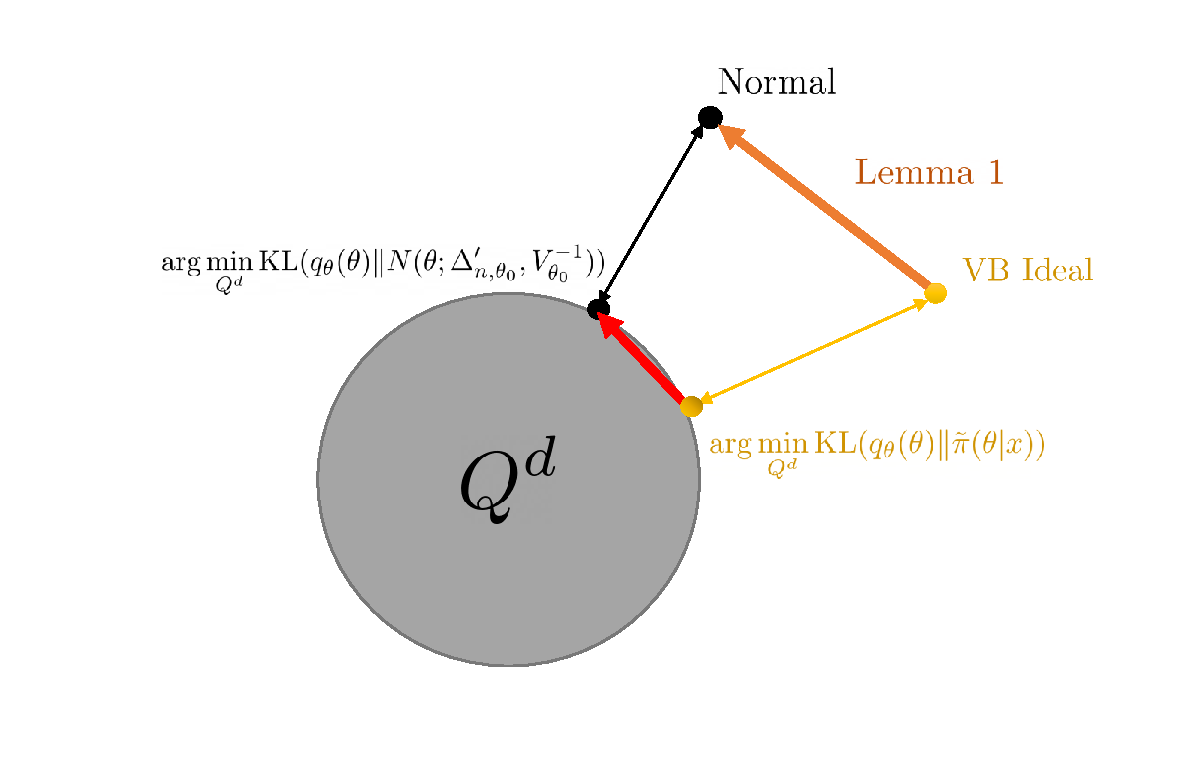
\includegraphics[width = 0.8\linewidth]{graphics/fig1.pdf}
	\label{lemma3fig}
	\caption{Schematic of Lemma \ref{lem3}. The red arrow indicates the convergence implied.}
\end{figure} 

\subsection{Connecting the VB Posterior}

\paragraph{} As mentioned before, we want to derive a BvM result on the global portion of the VB posterior, i.e., $q_{\theta}$. Recall the factorization from equation (8). We can expand the ELBO according to this:
\begin{gather*}
ELBO(q_\theta(\theta)q_z(z)) = \bbE_q[\log(p(\theta,z,x))] - \bbE_q[\log(q_{\theta}(\theta)q_z(z))] \\
= \bbE_{q}[\log(p(x, z|\theta)p(\theta)) - \log(q_{\theta}(\theta)q_z(z))] \\
= \int\int d\theta dz q_\theta(\theta)q_z(z) \log \left( \frac{p(\theta) p(x, z|\theta)}{q_{\theta}(\theta)q_z(z)} \right) \\
= \int d\theta q_{\theta}(\theta) \log \left(\frac{p(\theta)}{q_{\theta}(\theta)} \right) + \int d\theta q_{\theta}(\theta) \int dz q_z(z)\log \left(\frac{p(x,z|\theta)}{q_z(z)} \right)
\end{gather*}
In this form, we can use the strategy of profiling to obtain the optimal distribution $q_{\theta}$, viewing the local factor as a nuisance parameter. That is, if $q_z$ is viewed as fixed, we can derive
$$
q'_{\theta} = \arg\max_{Q^d} ELBO(q_{\theta}(\theta)q_z(z))
$$
%
Now, the factor $q^*_{\theta}$ of the global optimum, i.e., the VB posterior, is obtained simply by taking the maximum value of the ELBO with respect to $q_z$ first. That is,
\begin{equation}
\label{profileELBO}
q_{\theta}^*(\theta) = \arg \max_{Q^d} \left(\sup_{Q^n} ELBO(q_{\theta}(\theta)q_z(z)) \right)
\end{equation}
%
Note the inner supremum still takes on a different value for each $q_{\theta}$. If we denote the profiled ELBO $\sup_{Q^n} ELBO(q_{\theta}(\theta)q_z(z)) = ELBO_p(q_{\theta}(\theta))$, then we can rewrite Equation \ref{profileELBO} as $q_{\theta}^*(\theta) = \arg \max_{Q^d} ELBO_p(q_{\theta}(\theta))$, where
\begin{equation}
ELBO_p(q_{\theta}) = \sup_{Q^n} \int d\theta q_{\theta}(\theta) \left(- \log q_\theta(\theta) \log \left[ p(\theta) \exp \left[ \int dz q_{z}(z) \log\left( \frac{p(x,z|\theta)}{q_z(z)} \right)\right] \right] \right)
\end{equation}
We now have the notation to state the final lemma. 
\begin{lemma}[Lemma 4, \cite{Wang:2019:VBVM}]
	\label{lem4}
	Under some additional technical conditions on the variational densities in $Q^d$ (see exercise 1), we have that for any $q_{\theta}(\theta) \in Q^d$, 
	\begin{equation*}
	ELBO_p(q_{\theta}(\theta)) = -KL(q_{\theta}(\theta)\| \pi^*(\theta|x)) + C_n + o_p(1)
	\end{equation*}
	where $o_p(1)$ indicates that a remainder term converges to $0$ in probability under the probability measures in $Q^d$ and $C_n$ is bounded. 
\end{lemma}

This lemma suggests that the maximizer of the profiled ELBO, i.e., the VB posterior, is also the minimizer of the KL to the VB ideal. In view of Lemma \ref{lem3}, this is a profound result. The proof sketch of this Lemma is appealing and insightful. Notice that the KL divergence is to the VB ideal, which implicitly involves a maximization over $q$, much like the profiled ELBO. We can write the negative KL-divergence as
$$
 -KL(q_{\theta}(\theta)\| \pi^*(\theta|x)) = \int d\theta q(\theta)\log \left( \frac{p(\theta)\exp(M_n(\theta;x))}{q_{\theta}(\theta)} \right) + C_n
$$
%
where the constant $C_n$ is the log of the denominator in the VB ideal. Then,
\begin{equation}
\label{KLlem4}
-KL(q_{\theta}(\theta)\| \pi^*(\theta|x)) = 
\end{equation}
\begin{equation*}
\int d\theta q_{\theta}(\theta) \left(- \log q_\theta(\theta) + \log \left[ p(\theta) \exp \left[ \sup_{Q^n} \int dz q_{z}(z) \log\left( \frac{p(x,z|\theta)}{q_z(z)} \right)\right] \right] \right) + C_n
\end{equation*}
Notice that the term which depends on $q_{\theta}$ differs from the profiled ELBO only by the location of the supremum. Given a $q_{\theta}$, the profiled ELBO implicitly solves the optimization over $q_z$ once. Since the derivation involves solving the joint optimization over both $q_z$ and $q_{\theta}$, it is reasonable to expect that these are simultaneously determined. In equation \ref{KLlem4}, every value of $\theta$ in $q_{\theta}$ can result in a different optimal $q_z$ determining the supremum. To avoid this issue, if $q_{\theta}$ is restricted to be a point mass, then varying $\theta$ does not change the expression and the profiled ELBO and equation \ref{KLlem4} are equivalent. Recall that Lemma \ref{lem1} suggests the VB ideal converges to a point mass. Since the KL divergence between two distributions is infinite if the do not share the same support, the minimizer of the KL divergence to the VB ideal should also converge to a point mass. A portion of the proof is included as Exercise A.1. For a full technical justification, see the appendix in \cite{Wang:2019:VBVM}. 

\subsection{Main Result}
\paragraph{} Prior to stating the main result, we will discuss the chain of implications of the four lemmata above. In Lemma \ref{lem1}, we established the classical BvM result for the rescaled VB ideal, using an extension to misspecified models to account for the variational approximation. This is a precursor to the next two lemmata. We argued heuristically that this meant unscaled VB ideal converges to a point mass. In Lemma \ref{lem2}, we showed that the KL minimizer in the variational family to the VB ideal converges to the point mass at $\theta_0$, i.e., it is consistent. Lemma \ref{lem3} shows that the KL minimizer, or variational approximation to the scaled VB ideal and the variational approximation to a normal are equal in the limit in total variation. In other words, the result from Lemma \ref{lem1} survives the variational approximation on both terms. Finally, Lemma \ref{lem4} states that the maximizer of the ELBO converges to the variational approximation to the VB ideal. Combining with Lemma \ref{lem3} essentially gives the variational BvM result. We now state the main result. 

\begin{theorem}[Variational Bernstein von--Mises Theorem, Theorem 5 \cite{Wang:2019:VBVM}]
	\label{vbvm}
	Let $q^*_{\theta}$ denote the density of the variational approximation $Q^*_{\theta}$ to the posterior distribution of the global latent variables. Suppose the technical conditions of Lemma \ref{lem3} and Lemma \ref{lem4} hold. 
	\begin{enumerate}
		\item (Consistency) The following event occurs almost surely under the true probability measure $P_{\theta_0}$
		\begin{equation*}
		Q^*_{\theta}(\theta) \to \delta_{\theta_0}
		\end{equation*}
		in distribution. 
		\item (Asymptotic Normality) The VB posterior converges to the variational approximation of a normal distribution in total variation. Denote the scaled variational approximation by $\tilde{Q}_{\theta}$ with density $\tilde{q}_{\theta}(\tilde{\theta}) = q^*_{\theta}(\theta_0 + \delta_n\tilde{\theta}) |det(\delta_n)|$. Then, 
		\begin{equation*}
		\| \tilde{Q}_{\theta}  -
		\arg\min_{Q^d} \text{KL}(q_{\theta}(\theta)\| N(\theta; \Delta_{n, \theta_0}', V^{-1}_{\theta_0}))\|_{TV} \to 0
		\end{equation*}
	\end{enumerate}
\end{theorem}
	Recall that normal marginals are independent if and only if its covariance terms are 0. This special fact means that the mean-field variational family includes normal distributions, so long as the covariance matrix is diagonal. Indeed, we can show that
	\begin{equation}
	\label{meanfield}
	\arg\min_{Q^d} \text{KL}(q_{\theta}(\theta)\| N(\theta; \Delta_{n, \theta_0}', V^{-1}_{\theta_0})) = N(\theta; \Delta_{n, \theta_0}', V'^{-1}_{\theta_0})
	\end{equation}
	%
	where $V'_{\theta_0}$ is equal to $V_{\theta0}$ with all off-diagonal terms set to 0. This means that the mean-field scaled VB posterior converges to an uncorrelated normal distribution. The proof of equation \ref{meanfield} can be found in (\cite{Bishop::2006}, section 10.1). 
	
	\paragraph{}Although we restricted the exposition to the mean-field family, the authors emphasize that the results hold as long as lemmata \ref{lem1}-\ref{lem4} are satisfied. In particular, lemmata \ref{lem1} and \ref{lem4} are general in that the proof does not assume the mean-field. Lemma \ref{lem2} holds as long as the variational family at least includes the mean-field. In \cite{Wang:2019:VBVM}, the proof for lemma \ref{lem3} assumes the mean-field family, but it can also be shown for the full-rank Gaussian family. In other words, checking Theorem \ref{vbvm} for a variational family that is extended beyond the mean-field is equivalent to checking lemma \ref{lem3}. 
	



% open questions section
% !TEX root = ../main.tex

% open questions section

\section{Open questions and research directions}

%%%% appendix
\clearpage
\appendix

% exercises and problems
% !TEX root = ../main.tex

% Exercises section

\section{Exercises}

% any other appendix sections


% bibliography
\printbibliography

\end{document}